\chapter{Projektbeschreibung}
% noch mal Bezug nehmen auf das Projektplanungsdokument (nur das, was wirklich relevant
% für dieses Projekt ist)
\section{Ausgangslage und Problemstellung}
\section{Anforderungen an das Quiz}
\section{Methodik und Vorgehensweise}
% Grundsätzlich umfasst das Projektmanagement alle organisatorischen und führungsrelevanten Aufgaben
% sowie Techniken und Mittel zur operativen Durchführung, Überwachung und
% Unterstützung von Projekten.
% \footcite[Vgl.][3]{holzbaurNachhaltigesProjektmanagementVerantwortlichkeit2022}
% Insbesondere die Qualität eines Projekts ist abhängig
% von der Beschaffenheit des Projektmanagements.
% \footcite[Vgl.][52]{stoegerWirksamesProjektmanagementMit2019}
% Eine der Kerndisziplinen des
% Projektmanagements ist die Projektorganisation, welche Projektpläne,
% Dokumentationen für Projektmitarbeiter, eine Zeitplanung sowie
% die Verteilung von Aufgabenpaketen und jegliche weiteren Formen der
% Projektinfrastruktur umfasst.
% \footcite[Vgl.][53]{stoegerWirksamesProjektmanagementMit2019}
% Ein verbreiteter Ansatz der regelmäßigen Überprüfung der Projektorganisation
% stammt von Peter Drucker und besteht darin, in festgelegten Intervallen
% drei Kernfragen zu beantworten:
% \begin{itemize}
%     \item Ist die Projektorganisation so ausgerichtet, dass Nutzen für den Projektkunden gestiftet wird?\footcite[][57]{stoegerWirksamesProjektmanagementMit2019}
%     \item Stellt die Projektorganisation sicher, dass die Projektmitarbeiter ihre Aufgaben so erledigen können, dass der Zweck des Projekts erreicht wird?\footcite[][57]{stoegerWirksamesProjektmanagementMit2019}
%     \item Kann sich die Projektleitung mithilfe der Projektorganisation ihrer Kernaufgabe widmen – der Steuerung des Projekts?\footcite[][57]{stoegerWirksamesProjektmanagementMit2019}
% \end{itemize}
% \section{Projektplanung und Projektrollen}
% Zu Beginn eines jeden Projekts benötigt es eine Verteilung der Rollen und Verantwortlichkeiten innerhalb des Projekts.
% \footcite[Vgl.][89]{stoegerWirksamesProjektmanagementMit2019}
% In einem Projekt gibt es zahlreiche solcher Stakeholder, deren Identifikation und Management von entscheidender Bedeutung sind.
% Um dies effektiv zu handhaben, empfiehlt es sich, ein strukturiertes Schema zur Erfassung und Organisation dieser Stakeholder zu verwenden.
% Die Blaupause des benutzten Schemas für die Festlegung der Projektrollen und deren Verantwortlichkeiten ist in \textit{Anhang 1} zu finden.
% Die konkrete Zuordnung der Rollen und jeweils verantwortlichen Personen erfolgt hierbei bereits im Vorfeld der Projektplanung
% (siehe Tab. \ref{tab:rollen}).
% \begin{table}[H]
%     \centering
%     \begin{tabular}{|p{3.5cm}|p{4cm}|p{7cm}|}
%         \hline
%         \textbf{Rolle} & \textbf{Besetzung} & \textbf{Verantwortlichkeiten} \\
%         \hline
%         Auftraggeber & Michael Herwig & Auftragserteilung, Vorgabe und Kontrolle \\
%         & Prof. Kai Holzweißig & der Ziele, Abnahme des Projektergebnisses \\ 
%         & Lars Probst & \\
%         \hline
%         Projektleitung & Simon Spitzer & \begin{itemize}
%             \item Ziele der Auftraggeber in Teilziele und Arbeitspakete aufteilen
%             \item Aufgaben, Komeptenzen und Verantwortlichkeiten den Projektmitarbeitern zuordnen
%             \item Projektorganisation und -kommunikationswege festlegen (Jira, Discord, WhatsApp etc.)
%             \item Kommunikation mit Beteiligten (Sekreatariat, Studiengangsleiter etc.)
%             \item Umsetzung des Projektes überwachen und steuern
%             \item Berichterstattung an Auftraggeber
%         \end{itemize} \\
%         % Ziele der Auftraggeber in Teilziele und Arbeitspakete aufteilen \\
%         % & & Aufgaben, Komeptenzen und Verantwortlichkeiten der Projektmitarbeiter festlegen \\
%         % & & Projektorganisation und -kommunikationswege festlegen (Jira, Discord, WhatsApp etc.) \\
%         % & & Kommunikation mit Beteiligten (Sekreatariat, Studiengangsleiter etc.) \\
%         % & & Umsetzung des Projektes überwachen und steuern \\
%         % & & Berichterstattung an Auftraggeber \\
%         \hline
%         Projektmitarbeiter
%         & Simon Burbiel & grundsätzlich Ergebnisse gemäß den \\
%         & Lukas Großerhode & Arbeitspaketen umsetzen und \\
%         & Tim Keicher & verantworten \\
%         & David Stark & \\
%         & Simon Spitzer & \\
%         \hline
%         Externe Experten + & Prof. Kai Holzweißig & \\
%         Vertreter der DHBW & Tanja Schenk & \\
%         & Annette Voellmer & \\
%         & Nicole Bronder & \\
%         \hline
%     \end{tabular}
%     \caption{Rollen und Verantwortlichkeiten im Projekt.}\label{tab:rollen}
% \end{table}
% Besonders hierbei hervorzuheben ist die Kombination der Punkte 4 (externe Experten und Vertreter der DHBW),
% sowie 5. (Kunden). Die als „Experten“ fungierenden Mitarbeiter der DHBW teilen im Rahmen der durchzuführenden Interviews ihre Erfahrungen
% mit dem neuen Raumplanungsassisten und können in diesem Zuge auch auf Besonderheiten hinsichtlich der Nutzung und Bedienbarkeit des Programms
% hinweisen.
% Auch die Perspektiven derjenigen Mitarbeiter,
% welche noch keine Erfahrungen mit RAPLA haben sammeln können, sind von Bedeutung,
% da anhand dieser ebenso neue Erkenntnisse zur Gestaltung der Schulungsunterlagen und
% zur Zertifizierung gewonnen werden können. Des Weiteren ist als Besonderheit hervorzuheben,
% dass die Projektleitung auch operativ im Projekt mitarbeitet und
% sich nicht ausschließlich mit der Projektorganisation und dem Projektmanagement beschäftigt. Obwohl dies in der Literatur nicht in der Form
% angedacht ist, kann es für dieses Projekt unter Berücksichtigung von Umfang und fortlaufender iterativer Weiterentwicklung
% als sinnvoll angesehen werden.
% \footcite[Vgl.][89]{stoegerWirksamesProjektmanagementMit2019}

% \section{Interne Organisationsstruktur}
% Die interne Organisationsstruktur beinhaltet im Wesentlichen Wege der Kommunikation, Prüfungen hinsichtlich des Projektfortschritts,
% Verteilungen von Informationen sowie Möglichkeiten des kollaborativen Zusammenarbeitens.
% \footcite[Vgl.][460]{chenOrganizationalStructureDynamics2015}
% Bereits im Jahr 1996 war bekannt, dass hierfür computergetützte Lösungen vorteilhaft sind.
% \footcite[Vgl.][39]{easonDivisionLabourDesign1996}
% In dem RAPLA Schulungsprojekt wird hierfür das Programm „Jira Software“ benutzt.
% „Jira Software“ ist ein Kollaborationswerkzeug, welches den Nutzern unter anderem die Erstellung von Aufgaben-Übersichtstafeln,
% die Anlage von Listen mit über- und untergeordneten Aufgaben, die Zuordnung von Tätigkeiten zu bestimmten Personen
% sowie die Verwaltung einer Zeitleiste mit Fälligkeitsdaten ermöglicht.
% \footcites[Vgl.][1]{filionUsingAtlassianTools2017}[][87]{rehaPROJECTMANAGEMENTTOOLS2021}[][S. 32 ff.]{bradComparativeStudyAgile}
% Demnach ist dieses Werkzeug optimal für kollaborative Zusammenarbeiten geeignet. Weitere 
% Funktionalitäten und die konkreten Zuständigkeiten werden im Kapitel 
% „Arbeitspaketeplanung“ beschrieben. 

% Als zweites Kollaborationswerkzeug kommt Discord zum Einsatz. Es wird primär für den text- und sprachbasierten Informationsaustausch
% innerhalb des Teams genutzt. Zusätzlich werden dadurch
% Videotelefonate sowie das Teilen persönlicher Bildschirminhalte in Echtzeit ermöglicht.
% Ferner können dedizierte Text-Kanäle erstellt werden, die ebenfalls eine Unterstützung zum Teilen von Dokumenten anbieten.
% Des Weiteren gibt es Sprachkanäle, in welchen Regelmeetings virtuell abgehalten werden können. Eine beispielhafte Struktur eines sogenannten Community-Servers ist im Anhang 2 zu sehen.

% Es können viele Probleme entstehen, wenn vorab keine sinnvolle Verteilung der Aufgaben und Verantwortlichkeiten innerhalb des Teams erfolgt.
% \footcite[Vgl.][122]{suhandaRACIMatrixDesign2021}
% Um diesen Problemen entgegenzuwirken, wird im Rahmen dieses Projekts eine sogenannte \ac{RACI}-Matrix verwendet.
% Durch sie wird sichergestellt, dass alle Tätigkeiten und Rollen den entsprechenden Verantwortlichen zugewiesen werden und etwaige Klärungen hinsichtlich der Verantwortlichkeiten
% im späteren Projektverlauf vermieden werden können.
% \footcite[Vgl.][1]{farnettiOPTIMIZINGCOMMUNICATIONFLOWS2022}
% Die Grundprinzipien der \ac{RACI}-Matrix gehen auf die folgenden vier Buchstaben zurück:
% \begin{itemize}
%     \item \textbf{R}esponsible: Eine Person, welche für die Umsetzung einer Aufgabe verantwortlich ist.\footcite[Vgl.][4]{farnettiOPTIMIZINGCOMMUNICATIONFLOWS2022}
%     \item \textbf{A}ccountable: Eine Person, welche für das finale Endergebnis dem Auftraggeber gegenüber verantwortlich ist.\footcite[Vgl.][4]{farnettiOPTIMIZINGCOMMUNICATIONFLOWS2022}
%     \item \textbf{C}onsulted: Eine Person, welche bspw. aufgrund ihres Fachwissens in Entscheidungsprozesse involviert sein muss.\footcite[Vgl.][4]{farnettiOPTIMIZINGCOMMUNICATIONFLOWS2022}
%     \item \textbf{I}nformed: Eine Person, welche lediglich über den Fortschritt einer Aufgabe informiert werden muss.\footcite[Vgl.][4]{farnettiOPTIMIZINGCOMMUNICATIONFLOWS2022}
% \end{itemize}
% \begin{figure}[H]
%     \centering
%     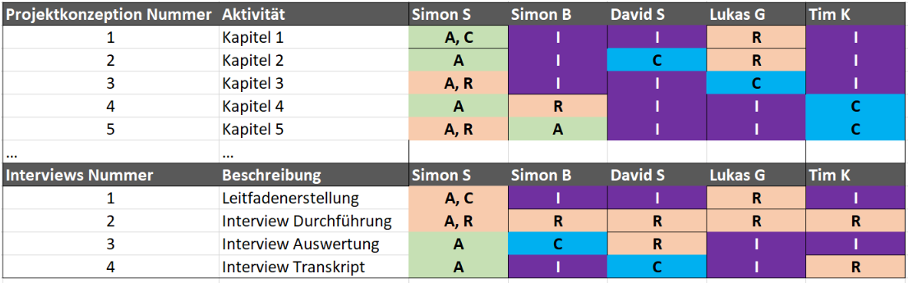
\includegraphics[width=0.9\linewidth]{graphics/raci.png}
%     \caption[Die \ac{RACI}-Matrix des Projekts.]{Die \ac{RACI}-Matrix des Projekts.}\label{abb:raci}
% \end{figure}
% \section{Regelmäßiger Austausch}
% Unabhängig davon, ob es sich um neue Entwicklungen, strategische Überlegungen, operative Angelegenheiten oder allgemeine Probleme handelt,
% ist es unerlässlich, diese Themen zu diskutieren. Dafür können entweder direkt die Verantwortlichen angesprochen werden, wenn diese
% existieren oder aber es wird in Regelmeetings über diese Punkte gesprochen. Jedoch führen ineffektive Regelmeetings zu verspäteten Entscheidungen,
% verschwendeten Ressourcen, verpassten Möglichkeiten und jeder Menge verlorener Zeit. 
% Eine Strategie und Grundsätze für Regelmeetings in einem Projekt zu etablieren und eine gewisse Qualität zu haben,
% scheint daher grundsätzlich vorteilhaft zu sein. Michael C. Mankins hat in seinem Artikel im „Harvard Business Review“-Journal „Stop Wasting Valuable Time” sieben Regeln
% aufgestellt, diese möglichst effektiv zu gestalten:
% \begin{itemize}
%     \item \textbf{Strategie und Operationen getrennt behandeln:} Strategische Themen benötigen mehr Zeit und sollten daher in separaten Meetings behandelt werden.
%     \item \textbf{Fokus auf Entscheidungen, nicht Diskussionen:} Qualität und Geschwindigkeit der Entscheidungsfindung verbessern, indem beispielsweise Dokumente im Voraus verschickt werden. Dies spart jedem Teilnehmer viel Zeit und auch die Gesamtlänge des Meetings wird verkürzt.
%     \item \textbf{Den wirklichen Wert jedes Tagesordnungspunktes messen:} Priorisieren der Tagesordnungspunkte nach ihrer Auswirkung auf den weiteren Verlauf des Projektes. Wichtige Punkte zuerst behandeln.
%     \item \textbf{Themen schnell von der Tagesordnung abhandeln:} Klare Zeitpläne festlegen, wann und wie Teilnehmer jedes Thema entscheiden, damit nicht zu viel Zeit auf einem Thema benötigt wird.
%     \item \textbf{Entscheidungen verbindlich machen:} Explizit vereinbaren, was in der Besprechung entschieden wurde. Entweder direkt während des Meetings festhalten oder eine Kommunikation im Nachgang senden.
% \end{itemize}
% Nachdem ein paar Grundsätze festgelegt werden, geht es an die Feinplanung der 
% Regelmeetings. Im 5. Semester ist ein wöchentliches Meeting jeden Donnerstag um 16:30Uhr vorgesehen.
% Der Zeitumfang beträgt dabei immer maximal eine Stunde. Wenn an diesem Tag Vorlesungen sind, wird werden die Treffen in Präsenz
% im Anschluss an die Vorlesung durchgeführt, in anderen Fällen finden diese per Videokonferenz statt. Zusätzlich zu diesem festgelegten Termin wird in der Vorlesungszeit
% des Kurses „Projektkonzeption“ über operative Tätigkeiten im Detail gesprochen und sich mit dem verantwortlichen Teammitgliedern abgestimmt,
% um die Entstehung von Dupletten oder unbehandelten Punkten am Ende des Projekts zu vermeiden.
